\documentclass[a4paper, 12pt]{article}
\usepackage{custom}
\usepackage{pgfplots}
\pgfplotsset{compat=1.18} % Impostare la compatibilità con la versione installata


%--------------------VARIABILI--------------------
\def\lastversion{v1.0}
\def\title{Piano di qualifica}
\def\date{17 Marzo 2025}
%------------------------------------------------

\begin{document}

\primapagina

\begin{registromodifiche}
        \lastversion & 17 Marzo 2025 &  & Enrico Bianchi & Release\\
    \hline
        v0.4 & 15 Marzo 2025 & Francesco Savio, Marko Peric & Enrico Bianchi & Aggiornamento \hyperref[sec:cruscotti_qualità]{cruscotti di valutazione della qualità}\\
    \hline
       v0.3 & 19 Febbraio 2025 & Enrico Bianchi & Francesco Savio & Aggiornamento \hyperref[sec:cruscotti_qualità]{cruscotti di valutazione della qualità}\\
    \hline
       v0.2 & 7 gennaio 2025 & Enrico Bianchi & Marko Peric & aggiunte tabelle delle metriche nelle sezioni \hyperref[subsec:obiettivi_processo]{Qualità di processo}, \hyperref[subsec:obiettivi_prodotto]{Qualità di prodotto}, aggiunta sezione \hyperref[subsec:processi_metriche]{Metriche per processo} \\
    \hline
        v0.1 & 23 dicembre 2024  & Enrico Bianchi & Marko Peric & Sezioni \hyperref[sec:introduzione_pq]{Introduzione documento}, \hyperref[sec:obiettivi_qualità]{Introduzione obiettivi di qualità}\\
    \hline
\end{registromodifiche}

 \tableofcontents

\newpage

\section{Introduzione}
\label{sec:introduzione}

\subsection{Scopo del documento}
\label{subsec:ScopoDelDocumento}
Il presente documento offre un'analisi approfondita dei casi d'uso e dei requisiti del progetto ArtificialQI, in linea con 
gli standard e le convenzioni dell'ingegneria del software. L'analisi è stata sviluppata a partire dal capitolato C1 
presentato dalla Proponente Zucchetti S.p.A., arricchita da una collaborazione attiva durante gli incontri dedicati. 
L'obiettivo principale è delineare le funzionalità e le caratteristiche dell'applicativo, fornendo una base solida per 
la successiva progettazione del sistema.

\subsection{Riferimenti}
\label{subsec:Riferimenti}

\subsubsection{Riferimenti normativi}
\label{subsubsec:RiferimentiNormativi}




\subsubsection{Riferimenti informativi}
\label{subsubsec:RiferimentiInformativi}

\documentclass[a4paper,12pt]{article}
\usepackage[T1]{fontenc}
\usepackage{custom}
\usepackage[nonumberlist,section=section]{glossaries}

%--------------------VARIABILI--------------------
\def\lastversion{v0.2}
\def\title{Glossario}
\def\date{31 dicembre 2024}
%------------------------------------------------

\renewcommand{\glspostdescription}{}

% Definizione dei termini del glossario

\newglossaryentry{A}{
    name = A,
    description = {}
}

\newglossaryentry{B}{
    name = B,
    description = {}
}

\newglossaryentry{C}{
    name = C,
    description = {}
}

\newglossaryentry{D}{
    name = D,
    description = {}
}

\newglossaryentry{E}{
    name = E,
    description = {}
}

\newglossaryentry{F}{
    name = F,
    description = {}
}

\newglossaryentry{G}{
    name = G,
    description = {}
}
\newglossaryentry{H}{
    name = H,
    description = {}
}

\newglossaryentry{I}{
    name = I,
    description = {}
}

\newglossaryentry{J}{
    name = J,
    description = {}
}

\newglossaryentry{K}{
    name = K,
    description = {}
}

\newglossaryentry{L}{
    name = L,
    description = {}
}

\newglossaryentry{M}{
    name = M,
    description = {}
}
\newglossaryentry{N}{
    name = N,
    description = {}
}

\newglossaryentry{O}{
    name = O,
    description = {}
}

\newglossaryentry{P}{
    name = P,
    description = {}
}

\newglossaryentry{Q}{
    name = Q,
    description = {}
}

\newglossaryentry{R}{
    name = R,
    description = {}
}

\newglossaryentry{S}{
    name = S,
    description = {}
}

\newglossaryentry{T}{
    name = T,
    description = {}
}

\newglossaryentry{U}{
    name = U,
    description = {}
}

\newglossaryentry{V}{
    name = V,
    description = {}
}

\newglossaryentry{W}{
    name = W,
    description = {}
}

\newglossaryentry{X}{
    name = X,
    description = {}
}

\newglossaryentry{Y}{
    name = Y,
    description = {}
}

\newglossaryentry{Z}{
    name = Z,
    description = {}
}






\newglossaryentry{Extend}{
    name=Extend,
    description={
    }
}

\newglossaryentry{Include}{
    name=Include,
    description={In UML (Unified Modeling Language), Include è un tipo di relazione utilizzato nei diagrammi di casi d'uso per 
    rappresentare un caso d'uso che include il comportamento di un altro caso d'uso. Questo tipo di relazione implica che un caso 
    d'uso principale esegue un altro caso d'uso come parte del proprio comportamento.
    La relazione Include viene utilizzata per separare la logica comune che può essere riutilizzata in diversi casi d'uso, 
    evitando la duplicazione del codice o della logica all'interno del sistema. Quando un caso d'uso "incluso" viene eseguito, 
    il caso d'uso "inclusivo" lo invoca sempre.
    }
}

\newglossaryentry{BGE 5 embedding}{
    name=BGE 5 embedding,
    description={
    }
}

\newglossaryentry{Bertino embedding}{
    name=Bertino embedding,
    description={BERTino Embedding si riferisce alle rappresentazioni vettoriali generate utilizzando il modello BERTino. Questi 
    embedding catturano le caratteristiche semantiche delle parole o delle frasi in italiano, facilitando compiti come il calcolo 
    della similarità tra testi e la ricerca semantica. BERTino offre una soluzione efficiente e specializzata per l'elaborazione 
    del linguaggio naturale in italiano, combinando l'efficacia dei modelli BERT con una struttura più leggera e prestazioni ottimizzate.
    }
}

\newglossaryentry{Nomic}{
    name=Nomic,
    description={
    }
}

\newglossaryentry{CSV}{
    name=CSV,
    description={CSV (Comma-Separated Values) è un formato di file utilizzato per memorizzare dati tabulari in forma di testo 
    semplice, in cui i valori sono separati da virgole. È ampiamente usato per lo scambio di dati tra applicazioni come fogli 
    di calcolo, database e software di analisi dati.
    }
}

\newglossaryentry{Embedding}{
    name=Embedding,
    description={L'embedding per il confronto tra stringhe è una tecnica che rappresenta le stringhe come vettori numerici in uno 
    spazio continuo, permettendo di calcolare la similarità tra di esse in modo efficiente.
    }
}

\newglossaryentry{Use Case}{
    name=Use Case,
    description={Un Use Case (Caso d'Uso) è una descrizione dettagliata di come un sistema interagisce con gli utenti (o altri 
    sistemi) per raggiungere un obiettivo specifico. È uno strumento fondamentale nell'analisi dei requisiti e aiuta a definire 
    il comportamento del software dal punto di vista dell'utente.
    }
}

\newglossaryentry{Database}{
    name=Database,
    description={Un database è un insieme organizzato di dati strutturati, memorizzati e gestiti in modo da consentire un accesso 
    efficiente, una facile manipolazione e un'integrità dei dati ottimale.
    }
}

\newglossaryentry{Dashboard}{
    name=Dashboard,
    description={Una dashboard è un'interfaccia utente grafica che visualizza informazioni chiave relative a un progetto o a 
    un sistema in modo sintetico e facilmente comprensibile.  Le dashboard sono utilizzate per monitorare lo stato di avanzamento, 
    identificare tendenze, individuare potenziali problemi e prendere decisioni informate.
    }
}

\newglossaryentry{OpenAPI 3.1}{
    name=OpenAPI 3.1,
    description={OpenAPI 3.1 è una specifica standardizzata per descrivere, documentare e definire API REST in modo leggibile 
    sia dagli esseri umani che dalle macchine. È l'evoluzione della specifica OpenAPI 3.0, sviluppata dalla OpenAPI 
    Initiative (OAI), con miglioramenti nella flessibilità e compatibilità con JSON Schema.
    }
}

\newglossaryentry{API REST}{
    name=API REST,
    description={Un'API REST (Representational State Transfer API) è un'interfaccia che permette la comunicazione tra sistemi 
    diversi attraverso il protocollo HTTP, seguendo i principi dell'architettura REST.
    }
}

\newglossaryentry{Committente}{
    name=Committente,
    description={Il committente è l'organizzazione o l'individuo che commissiona lo sviluppo di un sistema, prodotto o servizio 
    software a un fornitore. Il committente è colui che stabilisce i requisiti, le specifiche e 
    gli obiettivi che il prodotto finale deve soddisfare. 
    }
}

\newglossaryentry{Fornitore}{
    name=Fornitore,
    description={Il fornitore è un'organizzazione o un individuo che fornisce un prodotto software o un servizio software 
    a un'altra organizzazione o individuo (il cliente). Il fornitore è responsabile dello sviluppo, della consegna 
    e, in alcuni casi, della manutenzione del software o del servizio, in base ai requisiti e alle specifiche concordate con il 
    cliente.
    }
}

\newglossaryentry{Ciclo di vita}{
    name=Ciclo di vita,
    description={Ciclo di vita si riferisce all'insieme delle fasi che un sistema, un'applicazione o un componente software 
    attraversa dalla sua concezione fino al termine del suo utilizzo. Queste fasi descrivono il processo completo di sviluppo, 
    implementazione, gestione e dismissione del software o del sistema.
    }
}

\newglossaryentry{Stakeholder}{
    name=Stakeholder,
    description={Uno stakeholder è qualsiasi individuo, gruppo o organizzazione che ha un interesse diretto o indiretto in un progetto
    (portatore di interesse). Gli stakeholder sono essenziali perché definiscono i requisiti, gli obiettivi e i vincoli di un progetto, 
    influenzandone la direzione e il successo. }
}
\newglossaryentry{UML}{
    name=UML,
    description={Un diagramma UML (Unified Modeling Language) è una rappresentazione grafica utilizzata per modellare, 
    visualizzare, documentare e progettare sistemi software o processi. L'UML è uno standard internazionale che fornisce 
    un linguaggio visuale per descrivere sia la struttura che il comportamento di un sistema, rendendo più chiara e 
    condivisibile la progettazione tra sviluppatori, analisti, e stakeholder.}
}
\newglossaryentry{Best practices}{
    name=Best practices,
    description={Le best practices (in italiano, "migliori pratiche") sono un insieme di metodi, procedure, tecniche o regole 
    riconosciute come le più efficaci e affidabili per ottenere risultati ottimali in un determinato ambito. Queste pratiche 
    si basano su esperienze consolidate, studi, e casi di successo, e servono come guida per migliorare la qualità,
     l'efficienza e l'affidabilità di un processo o di un'attività.}
}
\newglossaryentry{Report}{
    name=Report,
    description={Un report è un documento o una rappresentazione strutturata di dati e informazioni, generato in modo automatico
     o manuale, con lo scopo di fornire una sintesi chiara e dettagliata su un determinato argomento, processo o sistema.}
}
\newglossaryentry{Label}{
    name=Label,
    description={Nna label (etichetta) è un identificatore utilizzato per rappresentare, descrivere o categorizzare un elemento,
     un dato o un'area specifica all'interno di un sistema, un programma o un'interfaccia. Il significato e l'utilizzo di una 
     label variano in base al contesto. }
}
\newglossaryentry{Caption}{
    name=Caption,
    description={una caption (didascalia) è un breve testo descrittivo associato a un elemento visivo o multimediale, 
    utilizzato per fornire informazioni contestuali, esplicative o identificative. Le caption aiutano gli utenti a comprendere
     meglio il contenuto a cui si riferiscono, migliorandone l'accessibilità e l'usabilità.}
}
\newglossaryentry{Sprint}{
    name=Sprint,
    description={Uno sprint è un'unità di lavoro a tempo determinato utilizzata nelle metodologie agili, in particolare nel
     framework Scrum, per sviluppare e rilasciare incrementi di un prodotto o progetto. Lo sprint rappresenta un intervallo
      di tempo fisso (solitamente da 1 a 4 settimane) durante il quale un team lavora per completare un set specifico di
       attività o obiettivi definiti nel backlog dello sprint.}
}
\newglossaryentry{Capitolato}{
    name=Capitolato,
    description={Un capitolato è un documento formale che definisce in modo dettagliato i requisiti, le specifiche e le
     condizioni tecniche, funzionali e organizzative di un progetto o di un sistema da sviluppare, acquisire o 
     implementare. Viene utilizzato come base di riferimento per lo sviluppo, la fornitura o la valutazione di soluzioni 
     informatiche.}
}
\newglossaryentry{IEEE 12207:1996}{
    name=IEEE 12207:1996,
    description={L'IEEE 12207:1996, noto anche come Software Life Cycle Processes, è uno standard internazionale sviluppato
     dall'Institute of Electrical and Electronics Engineers (IEEE), in collaborazione con l'ISO/IEC, che definisce un quadro
      di riferimento completo per i processi coinvolti nel ciclo di vita del software. Questo standard descrive tutte le
       attività necessarie per lo sviluppo, la gestione, la manutenzione e la dismissione di sistemi software.}
}
\newglossaryentry{Milestone}{
    name=Milestone,
    description={Una milestone (o pietra miliare) è un punto di riferimento significativo all'interno di un progetto o di un 
    ciclo di sviluppo software che segna il completamento di una fase importante o di un obiettivo specifico. Le milestone sono
     utilizzate per monitorare il progresso del progetto, per garantire che vengano rispettati i tempi e gli obiettivi
      prefissati e per facilitare la pianificazione delle fasi successive.}
}
\newglossaryentry{Baseline}{
    name=Baseline,
    description={Una baseline è una versione ufficiale e stabile di un sistema, di un software o di un progetto, che viene 
    utilizzata come punto di riferimento per tutte le successive modifiche e sviluppi. Una baseline rappresenta un insieme 
    di specifiche, documentazione, codice o configurazioni che sono stati approvati e che vengono considerati come "fissati"
     a un certo momento del ciclo di vita del progetto.}
}
\newglossaryentry{Repository}{
    name=Repository,
    description={un repository è un luogo centrale dove vengono archiviati e gestiti file, dati, codice sorgente o altre 
    risorse digitali, in modo strutturato e organizzato. Il repository permette di centralizzare e controllare l'accesso a
     questi file, facilitando il lavoro collaborativo e il versionamento. È uno strumento essenziale per la gestione del ciclo
      di vita del software e dei progetti, nonché per la conservazione e distribuzione dei dati.}
}
\newglossaryentry{Latex}{
    name=Latex,
    description={LaTeX è un linguaggio di markup e un sistema di preparazione di documenti, utilizzato principalmente per la 
    composizione di documenti scientifici, tecnici e accademici. LaTeX è ampiamente preferito in ambiti come la matematica, 
    la fisica, l'ingegneria e l'informatica grazie alla sua capacità di gestire complessi simboli matematici, formule, citazioni 
    bibliografiche e riferimenti incrociati.}
}
\newglossaryentry{RTB}{
    name=RTB,
    description={In ingegneria del software, RTB sta per "Reason to Believe" (Motivazione per Credere) ed è un concetto 
    utilizzato principalmente nell'ambito della valutazione della qualità e dell'affidabilità di un sistema software. 
    L'RTB rappresenta la giustificazione, la base o le evidenze che supportano la fiducia nella capacità di un software 
    di soddisfare i requisiti stabiliti.}
}
\newglossaryentry{Packages}{
    name=Packages,
    description={ il termine packages (pacchetti) si riferisce a un insieme di file o moduli software organizzati in una 
    struttura di directory e distribuiti come unità singola, destinati a facilitare la gestione, l'installazione e l'uso di
     componenti software. I pacchetti contengono tipicamente codice sorgente, librerie, configurazioni, documentazione e altre 
     risorse necessarie per l'implementazione di una funzionalità o applicazione specifica.}
}
\newglossaryentry{Pascal case}{
    name=Pascal case,
    description={Pascal Case è una convenzione di denominazione utilizzata in informatica, soprattutto nella programmazione, 
    in cui ogni parola che compone un nome o identificatore inizia con una lettera maiuscola, senza spazi o altri caratteri 
    separatori. In Pascal Case, la prima lettera di ogni parola, inclusa la prima, è maiuscola, e le parole sono concatenate 
    senza l'uso di underscore o altri simboli.}
}
\newglossaryentry{Configuration Item}{
    name=Configuration Item,
    description={Un Configuration Item (CI) è un elemento di un sistema informatico che viene gestito e monitorato come parte
     di un processo di gestione della configurazione. Un CI può essere qualsiasi componente hardware, software, documentazione,
      o altro elemento rilevante che influisce sul funzionamento di un sistema o di un progetto. Ogni CI è identificato in modo
       univoco e contiene informazioni relative alla sua configurazione, stato e versione.}
}
\newglossaryentry{Strategia di branching}{
    name=Strategia di branching,
    description={una strategia di branching (o strategia di ramificazione) è una pratica o un insieme di regole utilizzate nella
     gestione del controllo di versione del codice sorgente, in particolare quando si lavora con sistemi come Git. Essa
      definisce come e quando creare branch (rami) separati nel codice, in modo che i team di sviluppo possano lavorare in
       parallelo su diverse funzionalità, correzioni o versioni senza interferire con la versione principale del software.}
}
\newglossaryentry{Gitflow}{
    name=Gitflow,
    description={GitFlow è una strategia di branching che aiuta a gestire in modo strutturato lo sviluppo di 
    software, organizzando il lavoro in vari rami dedicati a specifici scopi, come lo sviluppo di funzionalità, la preparazione
     dei rilasci e la gestione delle correzioni di bug.}
}
\newglossaryentry{Codeline}{
    name=Codeline,
    description={Codeline è il termine utilizzato per riferirsi a una sequenza continua di versioni di codice sorgente che
     viene sviluppata e mantenuta all'interno di un sistema di controllo di versione. Una codeline rappresenta una "linea" di
      sviluppo del codice, che può evolversi con modifiche, miglioramenti e correzioni nel tempo.}
}
\newglossaryentry{Git}{
    name=Git,
    description={Git è un sistema di controllo versione distribuito open-source, utilizzato per gestire e tracciare le
     modifiche apportate a file e progetti, in particolare nel contesto dello sviluppo software. Permette a più sviluppatori
      di collaborare in modo efficace, tenendo traccia delle modifiche in un progetto e facilitando il lavoro su diverse
       versioni del codice.}
}
\newglossaryentry{Issue tracking system}{
    name=Issue tracking system,
    description={Un Issue Tracking System (ITS) è un software utilizzato per registrare, tracciare, gestire e risolvere le 
    problematiche, i bug, le richieste di funzionalità e altri tipi di "issue" (problemi) all'interno di un progetto o di 
    un'organizzazione. Questi sistemi sono essenziali per monitorare il progresso delle attività, assegnare compiti e 
    garantire che le problematiche vengano risolte in modo tempestivo ed efficiente.}
}
\newglossaryentry{Github}{
    name=Github,
    description={GitHub è una piattaforma di sviluppo software basata su Git, che fornisce un servizio di hosting per il 
    codice sorgente e supporta il controllo versione distribuito. GitHub permette di
     collaborare a progetti software in modo efficiente, mantenendo un repository centralizzato per il codice e facilitando 
     la gestione delle versioni, la revisione del codice e la collaborazione tra team.}
}


\newglossaryentry{Check list}{
    name=Check list,
    description={Una checklist è un elenco di elementi, attività o passaggi che devono essere verificati, completati o 
    controllati per assicurarsi che un processo o un'attività sia eseguito correttamente. Le checklist sono utilizzate per 
    garantire che tutte le operazioni necessarie siano state eseguite, riducendo il rischio di errori e dimenticanze.}
}
\newglossaryentry{Markup}{
    name=Markup,
    description={Markup si riferisce a un insieme di simboli o codici usati per annotare o strutturare il contenuto di un
     documento. Questi simboli o codici, noti come markup tags, indicano come il testo o gli altri contenuti devono essere
      trattati, visualizzati o interpretati da un programma.}
}
\newglossaryentry{PDF}{
    name=PDF,
    description={PDF (Portable Document Format) è un formato di file sviluppato da Adobe che consente di visualizzare,
     stampare e scambiare documenti in modo indipendente dal software, hardware e sistema operativo utilizzato. Il formato
      PDF è progettato per mantenere la formattazione originale di un documento, inclusi testo, immagini, grafica vettoriale,
       font e layout, in modo che appaia uguale su qualsiasi dispositivo o piattaforma.}
}
\newglossaryentry{Font}{
    name=Font,
    description={Un font è un insieme di caratteri tipografici che condividono uno stesso stile e dimensione. I font
     determinano l'aspetto visivo del testo, influenzando l'estetica e la leggibilità di un documento, di un sito web o di 
     un'applicazione. Ogni font include una varietà di simboli, lettere, numeri e segni di punteggiatura, tutti progettati 
     con lo stesso stile grafico.}
}
\newglossaryentry{TLShell}{
    name=TLShell,
    description={TLShell offre un modo sicuro e intuitivo per interagire con i dispositivi di rete, eseguire configurazioni 
    e monitorare lo stato dei dispositivi.}
}
\newglossaryentry{Radio button}{
    name=Radio button,
    description={Un radio button (o pulsante di opzione) è un tipo di controllo dell'interfaccia utente utilizzato nei moduli 
    e nelle applicazioni per permettere all'utente di selezionare una sola opzione da un gruppo di scelte predefinite.}
}
\newglossaryentry{Variabile di ambiente}{
    name=Variabile di ambiente,
    description={Una variabile di ambiente è una variabile dinamica che viene utilizzata dal sistema operativo e dai programmi
     in esecuzione per memorizzare informazioni di configurazione o parametri specifici relativi all'ambiente di esecuzione.
      Le variabili di ambiente forniscono un modo per configurare il comportamento di software, applicazioni e script senza
       dover modificare direttamente il codice.}
}
\newglossaryentry{IDE}{
    name=IDE,
    description={Un IDE (Integrated Development Environment) è un software che fornisce un insieme di strumenti integrati per
     facilitare lo sviluppo di applicazioni. Gli IDE sono progettati per aiutare i programmatori a scrivere, testare, eseguire
      e fare il debug del codice in modo più efficiente. Un IDE tipicamente combina diversi strumenti in un'unica interfaccia
       utente, semplificando il flusso di lavoro durante la scrittura del software.}
}
\newglossaryentry{Visual Studio Code}{
    name=Visual Studio Code,
    description={Visual Studio Code (VS Code) è un editor di codice sorgente open-source sviluppato da Microsoft, progettato
     per supportare una vasta gamma di linguaggi di programmazione e tecnologie. È leggero, altamente estensibile e dotato di 
     funzionalità avanzate per lo sviluppo di software.}
}
\newglossaryentry{Spell checkin}{
    name=Spell checkin,
    description={Spell checking (verifica ortografica) è il processo di controllo e correzione automatica degli
     errori di ortografia all'interno di un testo. Viene comunemente utilizzato in applicazioni come editor di testo, word
      processor, e-mail e strumenti di programmazione per rilevare parole scritte in modo errato o che non corrispondono a 
      quelle presenti in un dizionario di riferimento.}
}
\newglossaryentry{DVCS}{
    name=DVCS,
    description={DVCS (Distributed Version Control System) è un sistema di controllo di versione distribuito che consente a 
    più sviluppatori di lavorare su un progetto in modo collaborativo, tracciando e gestendo le modifiche al codice sorgente
     nel tempo. A differenza dei sistemi di controllo di versione centralizzati, in cui esiste un repository centrale, un DVCS
      consente a ciascun sviluppatore di avere una copia completa del repository, inclusa la cronologia delle modifiche, sul 
      proprio computer.}
}
\newglossaryentry{File system}{
    name=File system,
    description={Un file system è essenziale per la gestione dei dati su dispositivi di memorizzazione, permettendo di
     archiviare, recuperare e organizzare i file in modo sicuro e strutturato.}
}
\newglossaryentry{Fast-forward}{
    name=Fast-forward,
    description={Il termine fast-forward si riferisce a una situazione in cui una serie di operazioni o aggiornamenti viene
     applicata in modo diretto e senza conflitti, ovvero in modo che il risultato finale "avanzato" nel tempo sia una 
     progressione lineare senza la necessità di risolvere conflitti tra modifiche parallele.
    Nel contesto del controllo di versione (come Git), fast-forward indica una situazione in cui il ramo (branch) corrente
     può essere aggiornato semplicemente "avanzando" la sua punta (tip) al commit più recente di un altro ramo, senza dover 
     fare un "merge" (fusione) con risoluzione dei conflitti.}
}
\newglossaryentry{Console}{
    name=Console,
    description={La console è un'interfaccia utente che permette di interagire con un sistema operativo o un software tramite
     comandi testuali. Solitamente è un'applicazione software o a una finestra di terminale che permette agli utenti di inviare 
     comandi al sistema operativo o a un programma e ricevere risposte o output.}
}
\newglossaryentry{Keyword}{
    name=Keyword,
    description={ Keyword (parola chiave) si riferisce a una parola o a un termine che ha un significato speciale all'interno
     di un linguaggio di programmazione o di un sistema. Le parole chiave sono riservate e non possono essere utilizzate come
      identificatori (come nomi di variabili, funzioni o classi), poiché sono predefinite dal linguaggio per svolgere funzioni
       specifiche.}
}
\newglossaryentry{Current working directory}{
    name=Current working directory,
    description={La current working directory è la cartella in cui un programma o sistema operativo opera attualmente e svolge
     operazioni sui file.}
}
\newglossaryentry{ITS}{
    name=ITS,
    description={Un Issue Tracking System (ITS) è un software utilizzato per registrare, tracciare, gestire e risolvere le 
    problematiche, i bug, le richieste di funzionalità e altri tipi di "issue" (problemi) all'interno di un progetto o di 
    un'organizzazione. Questi sistemi sono essenziali per monitorare il progresso delle attività, assegnare compiti e 
    garantire che le problematiche vengano risolte in modo tempestivo ed efficiente.}
}
\newglossaryentry{Issue}{
    name=Issue,
    description={un issue è un termine generico utilizzato per riferirsi a un problema, un bug, una richiesta o una questione
     che deve essere risolta o gestita all'interno di un progetto software. Le issue possono riguardare vari aspetti dello
      sviluppo software, come difetti nel codice, funzionalità da implementare, miglioramenti da apportare o discussioni
       relative a decisioni progettuali.}
}
\newglossaryentry{Markdown}{
    name=Markdown,
    description={Markdown è un linguaggio di markup leggero che consente di scrivere testo formattato in modo semplice, con 
    la possibilità di convertirlo facilmente in HTML o altri formati, ed è ampiamente utilizzato per la scrittura di
     documentazione.}
}
\newglossaryentry{Pull request}{
    name=Pull request,
    description={Una pull request è un meccanismo di collaborazione in cui uno sviluppatore propone modifiche al codice, 
    che vengono esaminate e potenzialmente integrate nel progetto principale, consentendo il controllo della qualità e 
    la revisione collettiva del codice.}
}
\newglossaryentry{Diagramma di Gantt}{
    name=Diagramma di Gantt,
    description={Il diagramma di Gantt è uno strumento di pianificazione visiva utilizzato per rappresentare graficamente
     le attività di un progetto nel tempo. Ideato da Henry L. Gantt negli anni 1910, questo diagramma è uno dei più comuni
      metodi per il controllo e la gestione di progetti, ed è utilizzato principalmente in contesti di gestione dei progetti
       per visualizzare la sequenza, la durata e il progresso delle attività.}
}
\newglossaryentry{Project back-log}{
    name=Project back-log,
    description={Il project backlog (o backlog del progetto) è un elenco prioritizzato di attività, requisiti, funzionalità
     o task che devono essere completati in un progetto. Viene utilizzato principalmente nelle metodologie agili, come Scrum, 
     per gestire e pianificare il lavoro da svolgere durante lo sviluppo di un prodotto o di una soluzione. Ogni voce nel
      backlog rappresenta un elemento di lavoro che può essere un requisito del cliente, una correzione di bug, una funzionalità
       nuova o un miglioramento da implementare.}
}
\newglossaryentry{Sprint backlog}{
    name=Sprint backlog,
    description={Lo Sprint Backlog è un elenco delle attività, dei task e delle funzionalità che il team di sviluppo si impegna 
    a completare durante uno Sprint.  Lo Sprint Backlog deriva dal Product Backlog, che contiene tutte le attività necessarie
     per completare un intero progetto. Durante la pianificazione dello Sprint, il team seleziona gli elementi dal Product
      Backlog che possono essere completati entro la durata dello Sprint e li inserisce nello Sprint Backlog.}
}
\newglossaryentry{GitHub action}{
    name=GitHub action,
    description={Una GitHub Action è uno strumento di automazione che consente di eseguire flussi di lavoro (workflows)
     direttamente all'interno di un repository GitHub. Le GitHub Actions sono utilizzate per automatizzare compiti ripetitivi,
      come il testing del codice, il deployment (distribuzione), la compilazione, e altre attività legate al ciclo di vita del
       software. Queste azioni si integrano con GitHub, facilitando l'integrazione continua (CI) e la distribuzione continua
        (CD) nei progetti software.}
}
\newglossaryentry{Container}{
    name=Container,
    description={Un container è una tecnologia di virtualizzazione leggera che consente di eseguire applicazioni in ambienti 
    isolati e portabili, chiamati contenitori. A differenza delle macchine virtuali tradizionali, i container condividono il
     sistema operativo sottostante, ma sono separati a livello di processo, garantendo che le applicazioni all'interno di
      ciascun container non interferiscano tra loro. Questa isolazione consente di eseguire applicazioni in modo consistente
      su qualsiasi ambiente.}
}
\newglossaryentry{Workflow}{
    name=Workflow,
    description={Un workflow è una sequenza definita di attività, compiti o processi che vengono eseguiti per completare una 
    specifica operazione o obiettivo. I workflow possono essere automatizzati o manuali e sono utilizzati per coordinare, 
    ottimizzare e monitorare i flussi di lavoro all'interno di un sistema informatico, di un'applicazione o di 
    un'organizzazione.}
}
\newglossaryentry{Host}{
    name=Host,
    description={Un host è qualsiasi dispositivo o sistema che fornisce risorse, servizi o capacità di comunicazione in 
    una rete. Un host può essere un computer, un server, un dispositivo mobile, o qualsiasi altro dispositivo che possa
     connettersi a una rete e interagire con altri dispositivi o sistemi.}
}
\newglossaryentry{OS}{
    name=OS,
    description={OS sta per Operating System (sistema operativo), che è un software di base fondamentale per la gestione 
    delle risorse hardware e software di un computer o dispositivo. L'OS fornisce un'interfaccia tra l'utente e l'hardware,
     gestendo operazioni come l'esecuzione di programmi, la gestione della memoria, il controllo dei dispositivi di
      input/output, e la gestione dei file.}
}
\newglossaryentry{GitHub action marketplace}{
    name=GitHub action marketplace,
    description={Il GitHub Action Marketplace è una piattaforma integrata in GitHub che permette agli utenti di scoprire, 
    acquistare e utilizzare azioni GitHub (GitHub Actions) }
}
\newglossaryentry{YAML}{
    name=YAML,
    description={YAML (Yet Another Markup Language) è un formato di serializzazione dei dati, leggibile dall'uomo,
     utilizzato per rappresentare informazioni in modo strutturato. Viene spesso impiegato per configurazioni, scambi 
     di dati e definizione di strutture nei contesti di sviluppo software.}
}
\newglossaryentry{Personal Access Token}{
    name=Personal Access Token,
    description={Un Personal Access Token (PAT) è un tipo di token di autenticazione che viene utilizzato per accedere a 
    risorse protette su piattaforme e servizi, come GitHub, GitLab, o Azure DevOps, al posto di una password tradizionale.
     I PAT vengono generati dall'utente e possono essere utilizzati per autentificarsi in modo sicuro e automatizzato quando
      si interagisce con API o si eseguono operazioni come il push di codice o la gestione di repository.}
}
\newglossaryentry{Framework}{
    name=Framework,
    description={Un framework è un insieme di strumenti, librerie e convenzioni che forniscono una struttura
     predefinita per lo sviluppo di applicazioni software. Si tratta di una piattaforma che semplifica e standardizza il 
     processo di sviluppo, consentendo agli sviluppatori di concentrarsi sulla logica applicativa piuttosto che scrivere 
     codice da zero per ogni singola funzionalità di base.}
}
\newglossaryentry{Agile}{
    name=Agile,
    description={Agile in informatica è un insieme di metodologie e pratiche di sviluppo software che promuovono iterazioni
     rapide, adattabilità ai cambiamenti e una stretta collaborazione tra il team di sviluppo e i clienti. Il termine Agile si
      riferisce a un approccio che enfatizza la flessibilità, la trasparenza e il miglioramento continuo, con l'obiettivo
       di consegnare software di qualità in modo rapido e reattivo alle necessità del cliente.}
}
\newglossaryentry{Modello di sviluppo a periodi}{
    name=Modello di sviluppo a periodi,
    description={Il modello di sviluppo a periodi (o ciclo di vita del software iterativo e incrementale) è un approccio in
     informatica che suddivide il processo di sviluppo del software in periodi o iterazioni ripetute, in cui ogni periodo
      produce una versione parziale ma funzionante del sistema. Ogni ciclo o periodo include fasi di progettazione, sviluppo,
       testing e revisione, e alla fine di ogni periodo viene rilasciato un incremento delle funzionalità del software.}
}
\newglossaryentry{Feedback}{
    name=Feedback,
    description={Il feedback è il processo attraverso il quale i risultati o le risposte di un sistema, applicazione o processo
     vengono restituiti agli utenti, ai team di sviluppo o ad altri attori coinvolti, per informare, correggere o migliorare
      il funzionamento del sistema stesso. Il feedback può essere positivo (quando il risultato è conforme alle aspettative)
       o negativo (quando è necessario apportare modifiche o correzioni).}
}
\newglossaryentry{Way of working}{
    name=Way of working,
    description={Il termine "way of working" (WoW) in informatica si riferisce al modo in cui un team, un'organizzazione
     o un progetto opera, gestisce e coordina le proprie attività per raggiungere i propri obiettivi. Include le metodologie,
      le pratiche, gli strumenti, le comunicazioni e le procedure seguite nel corso dello sviluppo e della gestione del lavoro.}
}
\newglossaryentry{Kanban board}{
    name=Kanban board,
    description={La Kanban board è uno strumento visivo utilizzato per gestire e monitorare il flusso di lavoro in progetti,
     tipicamente in contesti di sviluppo software o gestione dei processi aziendali. È una rappresentazione grafica che aiuta
      i team a visualizzare le attività in corso, a tracciare il progresso e a identificare eventuali colli di bottiglia nel
       processo.}
}
\newglossaryentry{ISO 31000}{
    name=ISO 31000,
    description={ ISO 31000 è uno standard che fornisce un approccio sistematico, integrato e continuo per la gestione del
     rischio, aiutando le organizzazioni a identificare, valutare e gestire i rischi in modo efficace per raggiungere i
      propri obiettivi.}
}

\makenoidxglossaries
\glsaddall

\begin{document}

\primapagina

\begin{registromodifiche}\label{sec:Registro delle modifiche}
    v0.2 & 28 dicembre 2024  & Marko Peric & Francesco Savio & Sezione \hyperref[sec:Indice]{Indice}\\
\hline 
    v0.1 & 19 dicembre 2024  & Francesco Savio & Marko Peric & Sezioni \hyperref[sec:introduzione]{Introduzione},  \hyperref[sec:glossario]{Glossario}\\
\hline 
\end{registromodifiche}

\section*{Indice}
\label{sec:Indice}
\begin{itemize}
    \item \hyperref[sec:Registro delle modifiche]{Registro delle modifiche}
    \item \hyperref[sec:introduzione]{Introduzione}
    \item \hyperref[sec:glossario]{Glossario}
    \begin{itemize}
        \item \hyperref[sec:glossario]{\gls{A}}
        \item \hyperref[sec:glossario]{\gls{B}}
        \item \hyperref[sec:glossario]{\gls{C}}
        \item \hyperref[sec:glossario]{\gls{D}}
        \item \hyperref[sec:glossario]{\gls{E}}
        \item \hyperref[sec:glossario]{\gls{F}}
        \item \hyperref[sec:glossario]{\gls{G}}
        \item \hyperref[sec:glossario]{\gls{H}}
        \item \hyperref[sec:glossario]{\gls{I}}
        \item \hyperref[sec:glossario]{\gls{J}}
        \item \hyperref[sec:glossario]{\gls{K}}
        \item \hyperref[sec:glossario]{\gls{L}}
        \item \hyperref[sec:glossario]{\gls{M}}
        \item \hyperref[sec:glossario]{\gls{N}}
        \item \hyperref[sec:glossario]{\gls{O}}
        \item \hyperref[sec:glossario]{\gls{P}}
        \item \hyperref[sec:glossario]{\gls{Q}}
        \item \hyperref[sec:glossario]{\gls{R}}
        \item \hyperref[sec:glossario]{\gls{S}}
        \item \hyperref[sec:glossario]{\gls{T}}
        \item \hyperref[sec:glossario]{\gls{U}}
        \item \hyperref[sec:glossario]{\gls{V}}
        \item \hyperref[sec:glossario]{\gls{W}}
        \item \hyperref[sec:glossario]{\gls{X}}
        \item \hyperref[sec:glossario]{\gls{Y}}
        \item \hyperref[sec:glossario]{\gls{Z}}
    \end{itemize}
\end{itemize}


\section*{Introduzione}
\label{sec:introduzione}
Questo glossario contiene termini contenuti nei documenti creati dal gruppo Alt+f4 che potrebbero richiedere una spiegazione più esaustiva,
 la ricerca può essere fatta tramite la parola specifica utilizzando il comando Ctrl+f, oppure scorrendo il glossario in ordine alfabetico.

\label{sec:glossario}

\printnoidxglossaries

\end{document}

\section{Obiettivi di qualità}
\label{sec:obiettivi_qualità}
Questa sezione ha lo scopo di indicare le metriche utilizzate per l'accertamento della qualità dei processi impiegati nella realizzazione
del progetto e dei prodotti realizzati.
Le metriche indicate si suddividono in:
\begin{itemize}
    \item metriche di processo
    \item metriche di prodotto
\end{itemize} 
Ogni metrica avrà indicato il codice identificativo associato, la soglia minima di accettazione e la soglia che ci si auspica di raggiungere 
per accertare la qualità massima raggiungibile del processo o del prodotto.
Ogni metrica indicata nelle tabelle realizzate è descritta con maggiore completezza all'interno del processo di Quality Assurance nelle Norme di Progetto.

\subsection{Qualità di processo}
\label{subsec:obiettivi_processo}
La qualità di processo si riferisce all'efficacia con cui vengono implementati e gestiti i processi durante il ciclo di vita dello sviluppo software, 
con l'obiettivo di garantire che il prodotto finale soddisfi i requisiti prefissati. 
Per monitorare e migliorare i processi, vengono adottate metriche di processo, ovvero indicatori chiave che misurano l'efficienza, l'affidabilità 
e la conformità delle attività svolte. 
Questi parametri, selezionati dal team, consentono di identificare aree critiche, ottimizzare le procedure operative e migliorare la produttività complessiva. 
L'uso delle metriche di processo contribuisce al controllo della qualità e alla riduzione dei rischi associati a ritardi o difetti.


\begin{table}[H]
    \centering
    \begin{tabular}{| l | l | l | l |}
    \hline
    \textbf{Identificativo} & 
    \textbf{Nome} &
    \textbf{Valore ammissibile} &
    \textbf{Valore ottimo}\\
    \hline
        M.PC.PV & Planned Value & $\geq 0$ & $\leq BAC$ \\
    \hline
        M.PC.EV & Earned Value & $\geq 0$ & $\leq EAC$ \\
    \hline
        M.PC.AC & Actual Cost & $\geq 0$ & $\leq EAC$ \\
    \hline
        M.PC.SV & Schedule Variance & $\geq -15\%$ & $0\%$ \\
    \hline
        M.PC.CV & Cost Variance & $\geq -15\%$ & $0\%$ \\
    \hline  
        M.PC.VP & \makecell{Variazione del Piano \\ tra costo effettivo \\ e costo preventivato} & $\leq 20\%$ & $\leq 5\%$ \\
    \hline
        M.PC.EAC & Estimated at Completion & $\leq BAC+5\% BAC$ & $\leq BAC$ \\
    \hline
        M.PC.RMR & Risk Mitigation Rate & $\geq 75\%$ & $100\%$ \\
    \hline
        M.PC.MS & Metriche Soddisfatte & $\geq 75\%$ & $100\%$ \\
    \hline
    \end{tabular}
    \caption{Metriche di processo}
    \label{tab:metriche_processo} 
\end{table}

\subsection{Obiettivi del prodotto}
L'obiettivo del prodotto è permettere la valutazione automatica delle prestazioni di un Large Language Model su un \glossario{dataset} composto da un insieme di coppie domanda-risposta.
Il sistema permetterà la riduzione/eliminazione della verifica umana diminuendo i costi dei test delle prestazioni su questi modelli di linguaggio.
Il sistema prodotto può quindi essere usato per:
\begin{enumerate}
    \item Confrontare le prestazioni di diversi Large Language Model.
    \item Confrontare le implicazioni prestazionali di diverse scelte implementative di un Large Language Model.
\end{enumerate} 
Il prodotto verrà quindi utilizzato per prendere decisioni sull'integrazione e l'implementazione di Large Language Model.


\usepackage{eurosym}

\pgfmathsetmacro{\BAC}{11250.0}   

\pgfmathsetmacro{\SpesaPA}{1008.75}  
\pgfmathsetmacro{\SpesaEA}{1008.75}  
\pgfmathsetmacro{\PercTA}{0.1}  
\pgfmathsetmacro{\PercEA}{0.1} 

\pgfmathsetmacro{\SpesaPB}{445.0}  
\pgfmathsetmacro{\SpesaEB}{378.75 + \SpesaEA} 
\pgfmathsetmacro{\PercTB}{0.35}  
\pgfmathsetmacro{\PercEB}{0.3} 

\pgfmathsetmacro{\SpesaPC}{342.5}  
\pgfmathsetmacro{\SpesaEC}{617.5 + \SpesaEB} 
\pgfmathsetmacro{\PercTC}{0.55}  
\pgfmathsetmacro{\PercEC}{0.55} 

\section{Cruscotto di valutazione della qualità}
\subsection{M.PC.PV - Planned Value}

\begin{tikzpicture}
    \begin{axis}[
        width=12cm, height=8cm,
        ymin=-100, ymax=12000,
        xtick={1, 2, 3},
        xticklabels={Sprint 1, Sprint 2, Sprint 3},
        xlabel={},
        ylabel={Costo (\euro)},
        grid=major,
        scaled ticks=false,
        legend style={at={(0.5,1.1)}, anchor=south, legend columns=-1},
    ]
    \addplot coordinates {(1, \BAC*\PercTA) (2, \BAC*\PercTB) (3, \BAC*\PercTC)};
    \addlegendentry{Valore misurato}
    \addplot[red, thick] coordinates {(0, 0) (4, 0)};
    \addlegendentry{Valore ammissibile}
    \addplot[orange, thick] coordinates {(0, \BAC) (4, \BAC)};
    \addlegendentry{Valore ottimo}
    \end{axis}
\end{tikzpicture}

\subsection*{RTB}

\subsection*{PB}
\subsection{M.PC.EV - Earned Value}

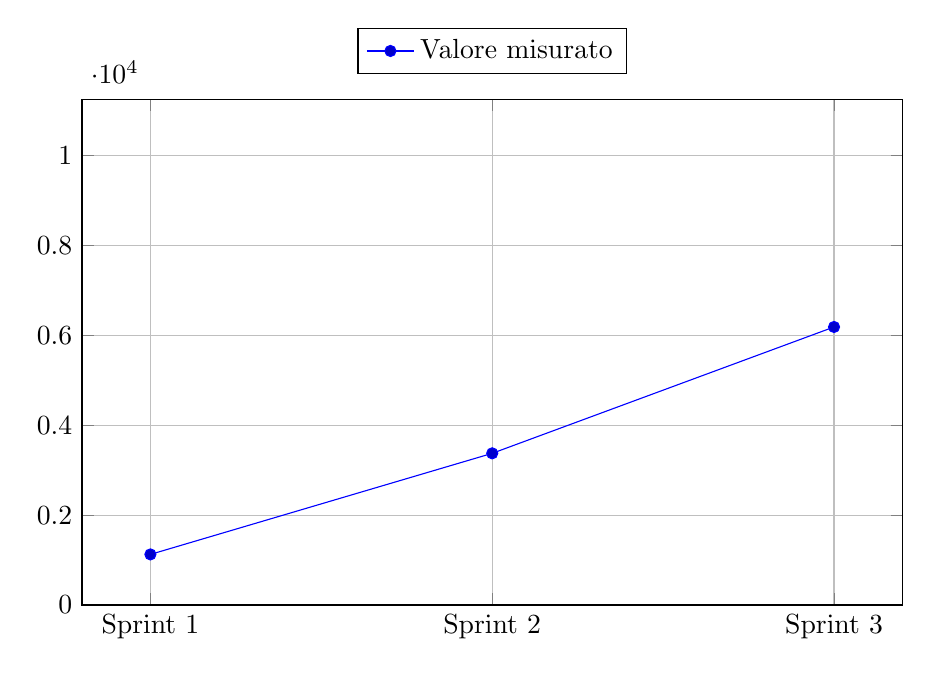
\begin{tikzpicture}
    \begin{axis}[
        width=12cm, height=8cm,
        ymin=0, ymax=11250,
        xtick={1, 2, 3},
        xticklabels={Sprint 1, Sprint 2, Sprint 3},
        xlabel={},
        ylabel={},
        grid=major,
        legend style={at={(0.5,1.05)}, anchor=south, legend columns=-1},
    ]
    \addplot coordinates {(1, 1125) (2, 3375) (3, 6187.5)};
    \addlegendentry{Valore misurato}
    \end{axis}
\end{tikzpicture}

\subsection*{RTB}

\subsection*{PB}
\subsection{M.PC.AC - Actual Cost}

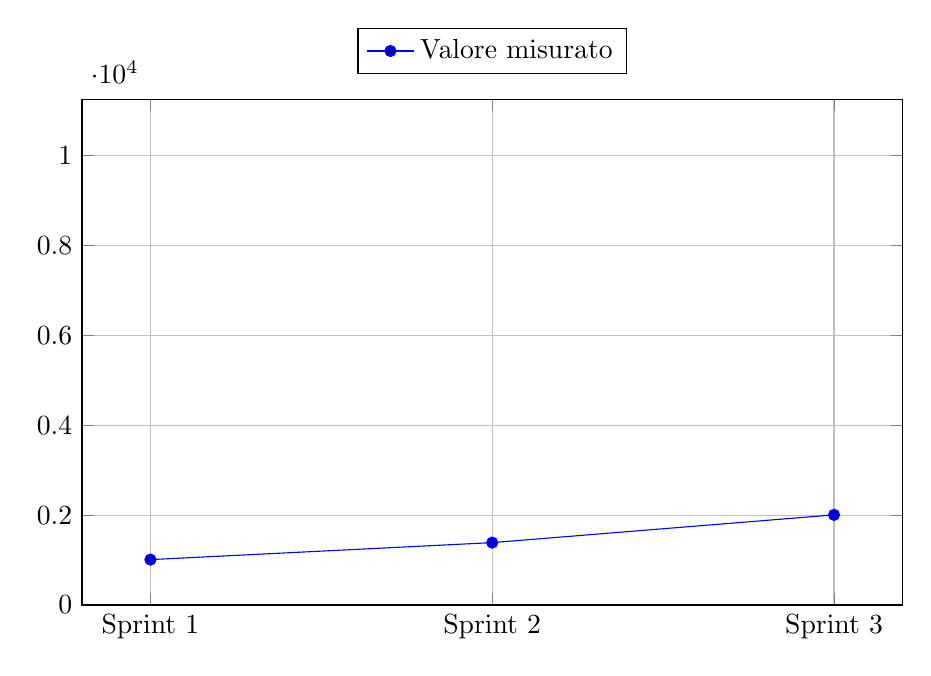
\begin{tikzpicture}
    \begin{axis}[
        width=12cm, height=8cm,
        ymin=0, ymax=11250,
        xtick={1, 2, 3},
        xticklabels={Sprint 1, Sprint 2, Sprint 3},
        xlabel={},
        ylabel={},
        grid=major,
        legend style={at={(0.5,1.05)}, anchor=south, legend columns=-1},
    ]
    \addplot coordinates {(1, 1008.75) (2, 1387.5) (3, 2005)};
    \addlegendentry{Valore misurato}
    \end{axis}
\end{tikzpicture}

\subsection*{RTB}

\subsection*{PB}
\subsection{M.PC.SV - Schedule Variance}

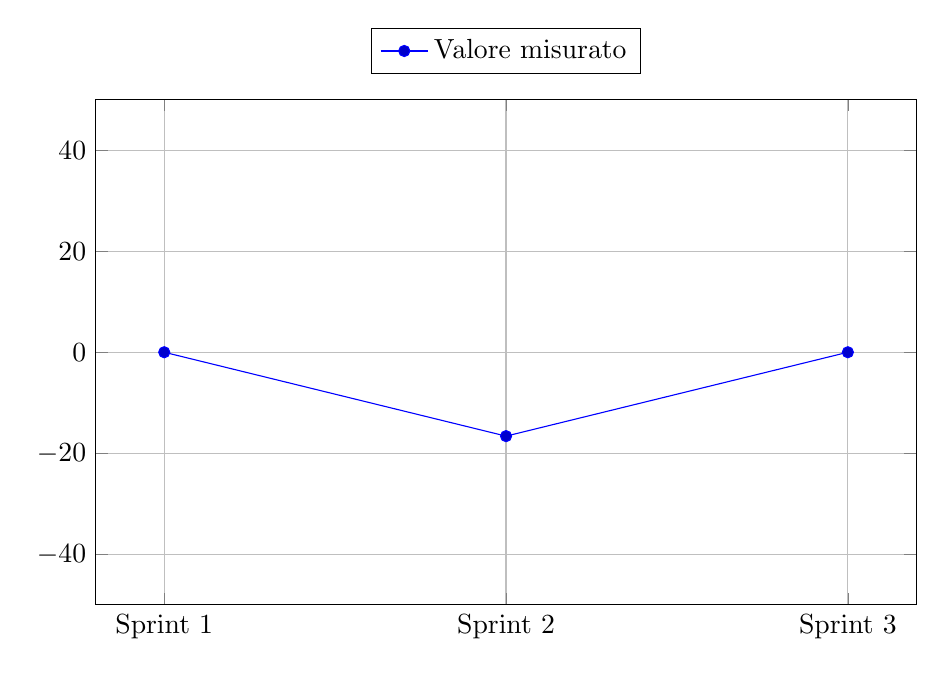
\begin{tikzpicture}
    \begin{axis}[
        width=12cm, height=8cm,
        ymin=-50, ymax=50,
        xtick={1, 2, 3},
        xticklabels={Sprint 1, Sprint 2, Sprint 3},
        xlabel={},
        ylabel={},
        grid=major,
        legend style={at={(0.5,1.05)}, anchor=south, legend columns=-1},
    ]
    \addplot coordinates {(1, 0) (2, -16.6) (3, 0)};
    \addlegendentry{Valore misurato}
    \end{axis}
\end{tikzpicture}

\subsection*{RTB}

\subsection*{PB}
\subsection{M.PC.CV - Cost Variance}

\begin{tikzpicture}
    \begin{axis}[
        width=12cm, height=8cm,
        ymin=-20, ymax=100,
        xtick={1, 2},
        xticklabels={Sprint 1, Sprint 2},
        xlabel={},
        ylabel={Percentuale (\%)},
        grid=major,
        scaled ticks=false,
        legend style={at={(0.5,1.1)}, anchor=south, legend columns=-1},
    ]

    \pgfmathsetmacro{\EVA}{\BAC*\PercEA} 
    \pgfmathsetmacro{\EVB}{\BAC*\PercEB}
    \pgfmathsetmacro{\EVC}{\BAC*\PercEC} 

    \addplot coordinates {(1, {((\EVA - \SpesaEA)/\EVA)*100}) (2, {((\EVB - \SpesaEB)/\EVB)*100}) (3, {((\EVC - \SpesaEC)/\EVC)*100})};
    \addlegendentry{Valore misurato}
    \addplot[red, thick] coordinates {(0, -15) (4, -15)};
    \addlegendentry{Valore ammissibile}
    \addplot[orange, thick] coordinates {(0, 0) (4, 0)};
    \addlegendentry{Valore ottimo}
    \end{axis}
\end{tikzpicture}

\subsection*{RTB}

\subsection*{PB}
\subsection{M.PC.VP - Variazione del Piano}

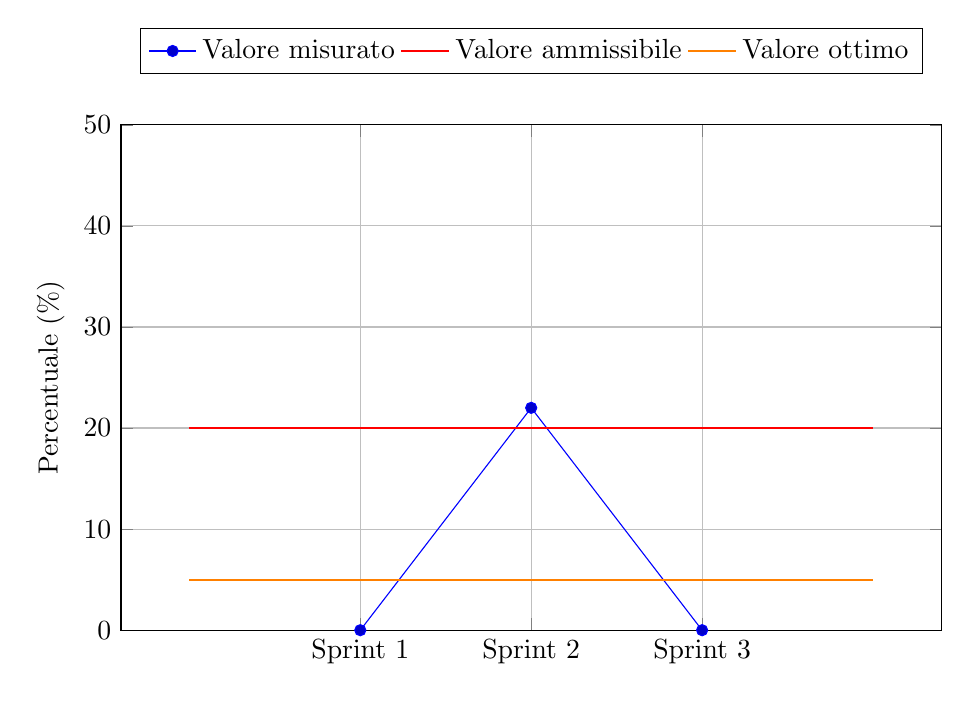
\begin{tikzpicture}
    \begin{axis}[
        width=12cm, height=8cm,
        ymin=0, ymax=50,
        xtick={1, 2, 3},
        xticklabels={Sprint 1, Sprint 2, Sprint 3},
        xlabel={},
        ylabel={Percentuale (\%)},
        grid=major,
        scaled ticks=false,
        legend style={at={(0.5,1.1)}, anchor=south, legend columns=-1},
    ]
    \addplot coordinates {(1, 0) (2, 22) (3, 0)};
    \addlegendentry{Valore misurato}
    \addplot[red, thick] coordinates {(0, 20) (4, 20)};
    \addlegendentry{Valore ammissibile}
    \addplot[orange, thick] coordinates {(0, 5) (4, 5)};
    \addlegendentry{Valore ottimo}
    \end{axis}
\end{tikzpicture}

\subsection*{RTB}

\subsection*{PB}
\subsection{M.PC.EAC - Estimated At Completition}

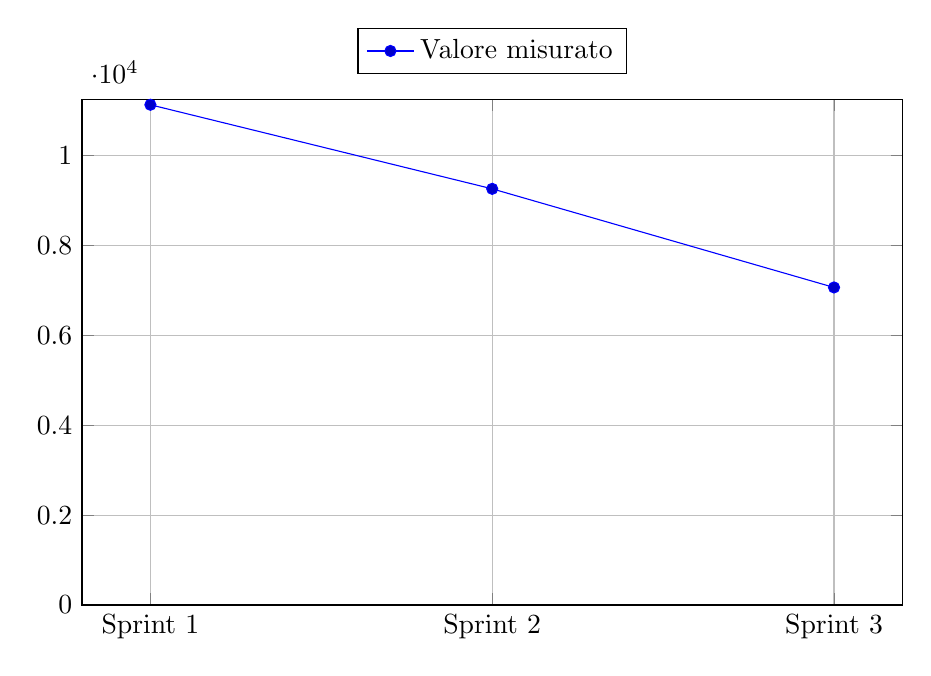
\begin{tikzpicture}
    \begin{axis}[
        width=12cm, height=8cm,
        ymin=0, ymax=11250,
        xtick={1, 2, 3},
        xticklabels={Sprint 1, Sprint 2, Sprint 3},
        xlabel={},
        ylabel={},
        grid=major,
        legend style={at={(0.5,1.05)}, anchor=south, legend columns=-1},
    ]
    \addplot coordinates {(1, 11133.75) (2, 9262.5) (3, 7067.5)};
    \addlegendentry{Valore misurato}
    \end{axis}
\end{tikzpicture}

\subsection*{RTB}

\subsection*{PB}
\subsection{M.PC.RI - Rischi Inattesi}

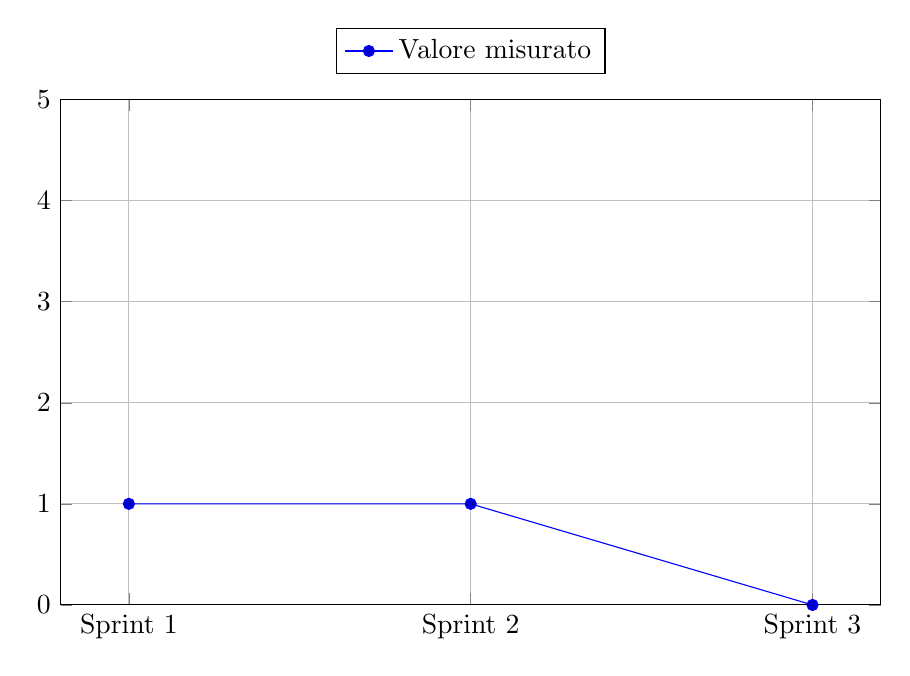
\begin{tikzpicture}
    \begin{axis}[
        width=12cm, height=8cm,
        ymin=0, ymax=5,
        xtick={1, 2, 3},
        xticklabels={Sprint 1, Sprint 2, Sprint 3},
        xlabel={},
        ylabel={},
        grid=major,
        legend style={at={(0.5,1.05)}, anchor=south, legend columns=-1},
    ]
    \addplot coordinates {(1, 1) (2, 1) (3, 0)};
    \addlegendentry{Valore misurato}
    \end{axis}
\end{tikzpicture}

\subsection*{RTB}

\subsection*{PB}
\subsection{M.PC.RMR - Risk Mitigation Rate}

\begin{tikzpicture}
    \begin{axis}[
        width=12cm, height=8cm,
        ymin=0, ymax=5,
        xtick={1, 2, 3},
        xticklabels={Sprint 1, Sprint 2, Sprint 3},
        xlabel={},
        ylabel={},
        grid=major,
        legend style={at={(0.5,1.05)}, anchor=south, legend columns=-1},
    ]
    \addplot coordinates {(1, 50) (2, 100), (3, 100)};
    \addlegendentry{Valore misurato}
    \end{axis}
\end{tikzpicture}

\subsection*{RTB}

\subsection*{PB}
\subsection{M.PC.MS - Metriche Soddisfatte}

\begin{tikzpicture}
    \begin{axis}[
        width=12cm, height=8cm,
        ymin=0, ymax=100,
        xtick={1, 2, 3},
        xticklabels={Sprint 1, Sprint 2, Sprint 3},
        xlabel={},
        ylabel={},
        grid=major,
        legend style={at={(0.5,1.05)}, anchor=south, legend columns=-1},
    ]
    \addplot coordinates {(1, 100) (2, 100), (3, 100)};% ci vogliono prima i valori ammissibili e non, non sono sicuro della formula scritta su RTB/DocumentiInterni/NormeDiProgetto/Sezioni/ProcessiDiSupporto/Sottosezioni/AccertamentoQualità.tex riguardo le MetricheSoddisfatte
    \addlegendentry{Valore misurato}
    \end{axis}
\end{tikzpicture}

\subsection*{RTB}

\subsection*{PB}
%\subsection{M.PR.PRM - Percentuale Requisiti Obbligatori Soddisfatti}

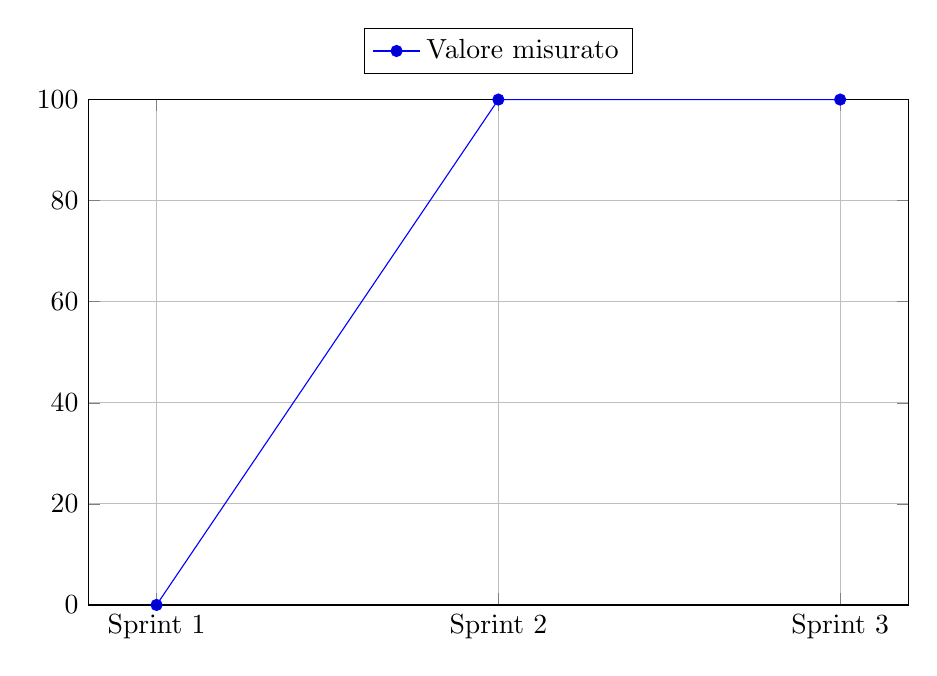
\begin{tikzpicture}
    \begin{axis}[
        width=12cm, height=8cm,
        ymin=0, ymax=100,
        xtick={1, 2, 3},
        xticklabels={Sprint 1, Sprint 2, Sprint 3},
        xlabel={},
        ylabel={},
        grid=major,
        legend style={at={(0.5,1.05)}, anchor=south, legend columns=-1},
    ]
    \addplot coordinates {(1, 0) (2, 100) (3, 100)};
    \addlegendentry{Valore misurato}
    \end{axis}
\end{tikzpicture}

\subsection*{RTB}

\subsection*{PB}
%\subsection{M.PR.PRD - Percentuale Requisiti Desiderabili Soddisfatti}

\begin{tikzpicture}
    \begin{axis}[
        width=12cm, height=8cm,
        ymin=0, ymax=100,
        xtick={1, 2, 3},
        xticklabels={Sprint 1, Sprint 2, Sprint 3},
        xlabel={},
        ylabel={},
        grid=major,
        legend style={at={(0.5,1.05)}, anchor=south, legend columns=-1},
    ]
    \addplot coordinates {(1, 0) (2, 50), (3, 100)};
    \addlegendentry{Valore misurato}
    \end{axis}
\end{tikzpicture}

\subsection*{RTB}

\subsection*{PB}
%\subsection{M.PR.PRO - Percentuale Requisiti Opzionali Soddisfatti}

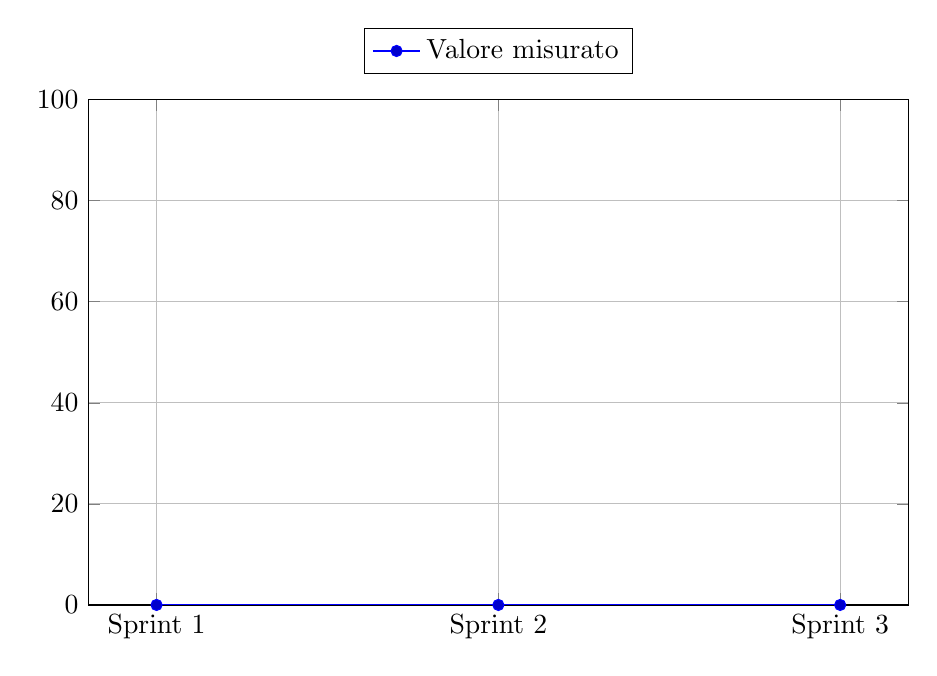
\begin{tikzpicture}
    \begin{axis}[
        width=12cm, height=8cm,
        ymin=0, ymax=100,
        xtick={1, 2, 3},
        xticklabels={Sprint 1, Sprint 2, Sprint 3},
        xlabel={},
        ylabel={},
        grid=major,
        legend style={at={(0.5,1.05)}, anchor=south, legend columns=-1},
    ]
    \addplot coordinates {(1, 0) (2, 0) (3, 0)};
    \addlegendentry{Valore misurato}
    \end{axis}
\end{tikzpicture}

\subsection*{RTB}

\subsection*{PB}
\subsection{M.PR.CO - Correttezza Ortografica}

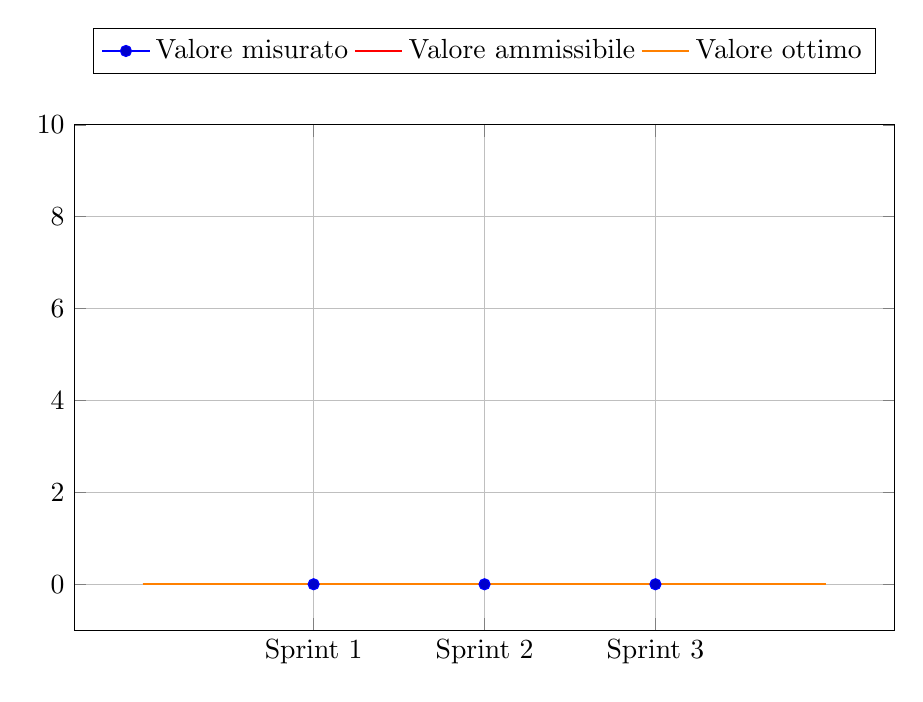
\begin{tikzpicture}
    \begin{axis}[
        width=12cm, height=8cm,
        ymin=-1, ymax=10,
        xtick={1, 2, 3},
        xticklabels={Sprint 1, Sprint 2, Sprint 3},
        xlabel={},
        ylabel={},
        grid=major,
        scaled ticks=false,
        legend style={at={(0.5,1.1)}, anchor=south, legend columns=-1},
    ]
    \addplot coordinates {(1, 0) (2, 0) (3, 0)};
    \addlegendentry{Valore misurato}
    \addplot[red, thick] coordinates {(0, 0) (4, 0)};
    \addlegendentry{Valore ammissibile}
    \addplot[orange, thick] coordinates {(0, 0) (4, 0)};
    \addlegendentry{Valore ottimo}
    \end{axis}
\end{tikzpicture}

\subsection*{RTB}

\subsection*{PB}



\end{document}